\documentclass{article}
\usepackage{graphicx} % Required for inserting images
\usepackage{float}
\usepackage{polyglossia} % used to display different languages
\usepackage{enumitem}
\usepackage{nameref}
\usepackage{fontspec}

% Path directory of images we want to import
\graphicspath{{./mockup-screens/flight-management}}

\setdefaultlanguage{greek}
\setotherlanguage{english}
\newfontfamily\greekfont{Arial}

\hfuzz=5.002pt 

\usepackage{fancyhdr} % used for custom headers

\pagestyle{fancy} % allow the creation of custom headers
\fancyhf{} % clear existing footers and headers
\setlength{\headheight}{1cm}
\rhead{
	SkyOps
	
\includegraphics[height=0.8cm, keepaspectratio]{image.png}
}

\title{
	
\includegraphics[height=1cm, keepaspectratio]{image.png}
	SkyOps
}
\author{
	Χρήστος Καπετανάκης 1103828 \\
	Ανδρέας Κρητικός 1104781 \\
	Γιώργος Τεμπονέρας 1104775 \\
	Ελευθερία Γιαννοπούλου 0000000 \\
	Αλέξης Λούμπαρδης 1051948
}

\date{} % date displayed underneath title

\setlength{\parskip}{16pt}


\begin{document}
	
	\maketitle
	
	\section{Σκοπός Εφαρομογής}
	Σκοπός του συστήματος SkyOps είναι να βοηθήσει τις αεροπορικές 
	εταιρείες να διαχειρίζονται αποτελεσματικά τις δραστηριότητές τους, 
	συμπεριλαμβανομένων των οικονομικών αναφορών, της διαχείρισης των εργαζομένων, 
	του προγραμματισμού πτήσεων και της βελτιστοποίησης των δρομολογίων. Το σύστημα 
	έχει σχεδιαστεί για να απλουστεύει τις περίπλοκες διαδικασίες που απαιτούνται 
	για τη διαχείριση μιας αεροπορικής εταιρείας, εξασφαλίζοντας την αποδοτικότητα 
	του κόστους, την αποτελεσματική χρήση των πόρων και την παροχή υπηρεσιών υψηλής 
	ποιότητας.
	
	\section{Βασικές Λειτουργίες}
	\subsection{Διαχείριση Πτήσεων}
	
	Το σύστημα επιτρέπει στους υπαλλήλους των αεροπορικών εταιρειών να διαχειρίζονται όλες τις πτήσεις τους:
	\begin{enumerate}
		\item Δημιουργία, επαναδρομολόγηση και ακύρωση πτήσεων. 
		\item Το σύστημα κάνει ελέγχους για το αν κάθε πτήση είναι έφικτη με τα στοιχεία που έχουν εισαχθεί από τον χρήστη ώστε να αποφεύγονται λάθοι, π.χ. το αεροπλάνο θα προλάβει να εξυπηρετήση αυτήν την πτήση αν είχε πριν μια άλλη?
		\item Ανάθεση αεροσυνοδών, πιλότων και μενού φαγητών στις πτήσεις.
		\item Αυτόματος υπολογισμός βασικών στοιχείων όπως διάρκεια πτήσης και χωρητικότητα πτήσης.
		\item Εύκολος τρόπος να βλέπει ο χρήστης της πτήσεις βάση συγκεκριμμένων παραμέτρων
		\item Υποστίριξη ειδών πτήσεων για επιβάτες, εμπόρευμα ή για πτήσης επανατοποθέτησης αεροσκάφων
	\end{enumerate}

	Στο σχήμα \ref{screen:flight-view} παρουσιάζεται η οθόνη που σου δείχνει όλες τις πτήσεις που περιέχει το σύστημα.
	Δίνει κάποια βασικά στοιχεία για να ξέρει ο χρήστης περίπου ποιές πτήσεις έχουν στοιχεία που τους λοίπουν και
	πτήσεις που δεν μπορούν να πραγματοποιηθούν γιατί κάτι έχει προκύψει. Επίσης του δίνει την δυνατότητα να επιλέξει
	μια πτήση. 
	
	Στο σχήμα \ref{screen:flight-details} παρουσιάζει στον διαχειριστή της εταιρίας δείχνει όλα τα στοιχεία της πτήσης
	που έχει καταγραφεί. Επίσης παράγει αυτόματα κάποια στοιχεία όπως το χρόνο της πτήσης και την απόσταση μεταξύ 
	αεροδρομίων.

	Στο σχήμα \ref{screen:Edit-Flight} επιτρέπει στον διαχειριστή της εταιρίας να αλλάξει κάποια στιοχεία της πτήσης
	όπως το προσωπικό και το αεροπλάνο και το ο αριθμός της πτήσης. Όμως δεν μπορεί να αλλάξει τίποτα άλλο γιατί
	θα αλλάξει τελείως η πτήση. Οπότε αναγκάζουμε τον χρήστη να ακυρώσει την πτήση αν θέλει να κάνει άλλες αλλαγές.
	Αυτό γίνεται γιατί π.χ. δεν μπορεί να αλλάξεις μια πτήση που αντί να προσγειώσει Αθήνα πάει Λονδίνο γιατί θεωρείται
	άλλη πτήση και οι επιβάτες δεν θα θέλουν να πάνε εκεί.

	Στο σχήμα \ref{screen:Flight-Reschedule} μας επιτρέπει να αλλάξουμε την ώρα της πτήσης. Για την ευκολία του χρήστη
	του έχουμε δώσει της προηγούμενες 2 πτήσεις και τις επόμενες 2. Με βάση αυτό μπορεί ο χρήστης να αλλάξει την ώρα
	πτήσης με τέτοιον τρόπο ώστε να μην επηρεάζει το υπόλοιπο δρομολόγιο. 

	\begin{figure}[H]
		\centering
		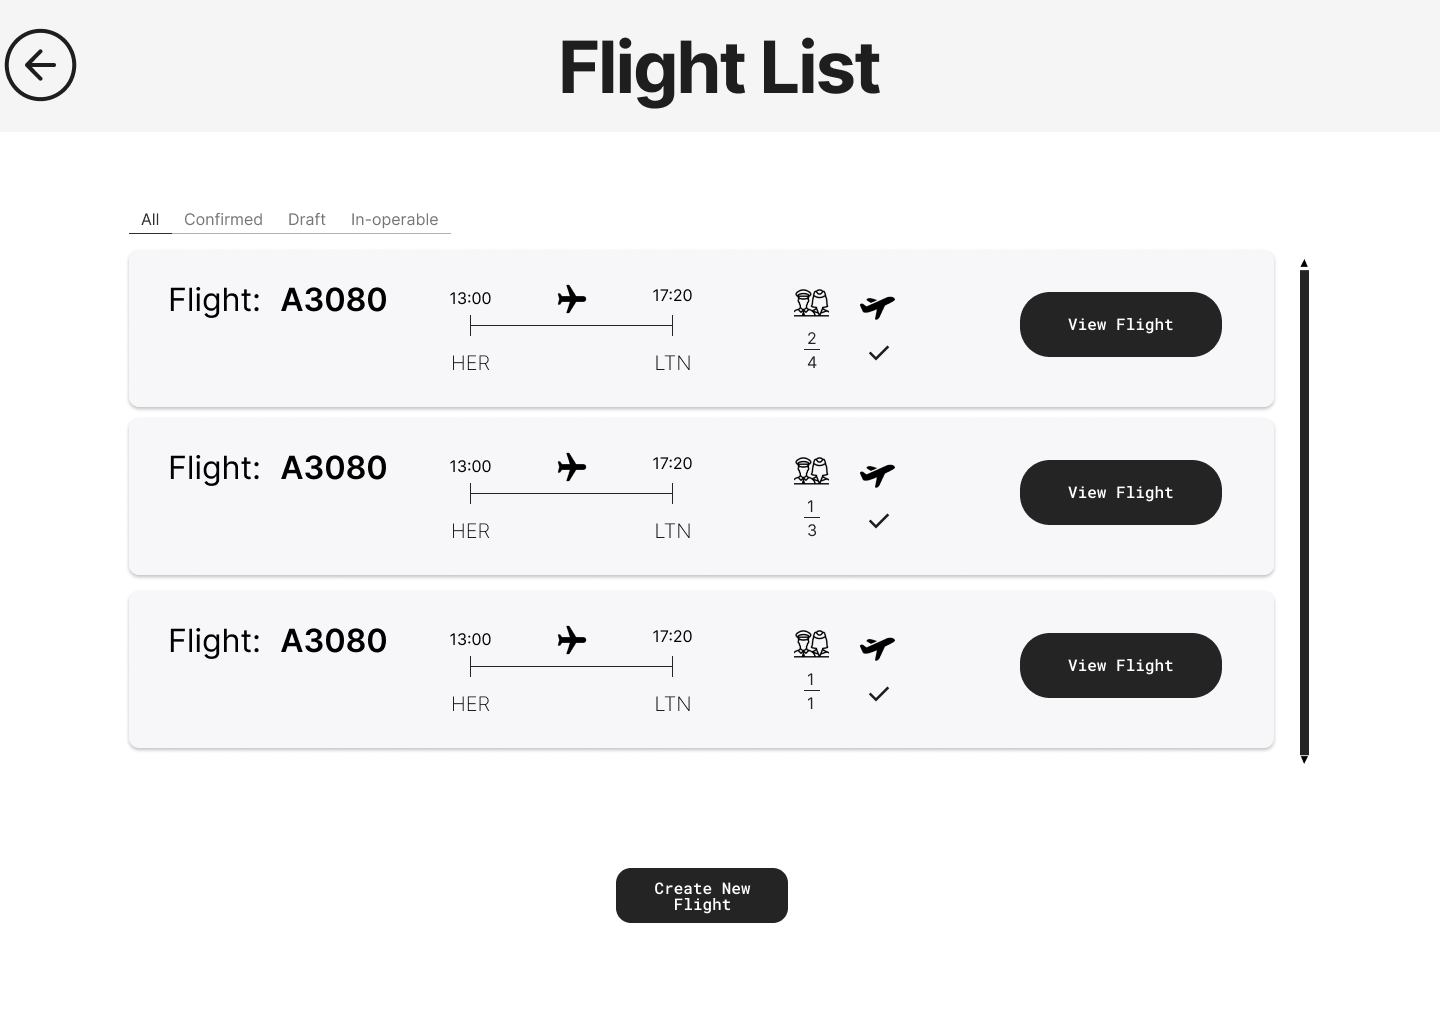
\includegraphics[width=0.75\textwidth]{../mockup-screens/flight-management/flight-list.png}
		\caption{Flight List}
		\label{screen:flight-view}
	\end{figure}

	\begin{figure}[H]
		\centering
		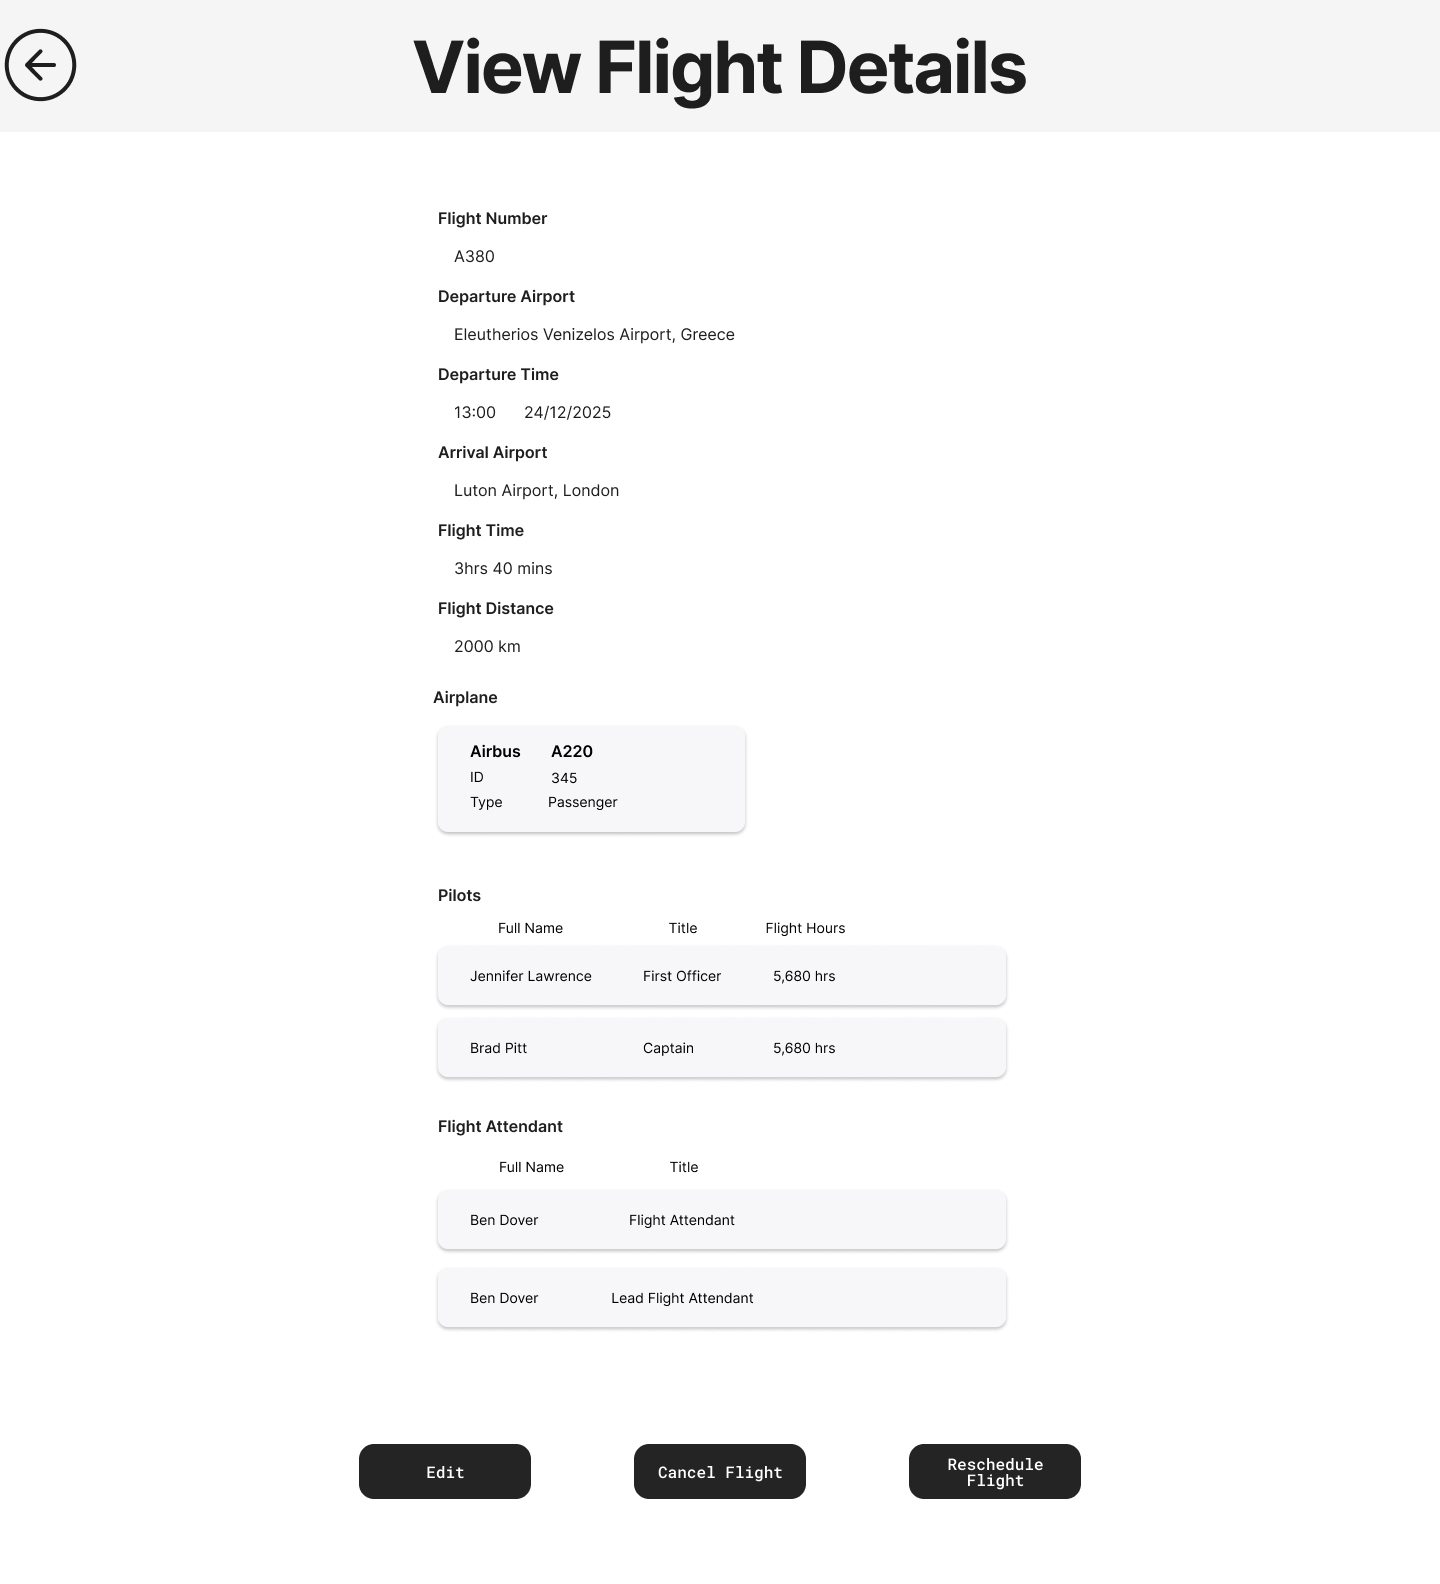
\includegraphics[width=0.75\textwidth]{../mockup-screens/flight-management/Flight-Details.png}
		\caption{Flight Details}
		\label{screen:flight-details}
	\end{figure}

	\begin{figure}[H]
		\centering
		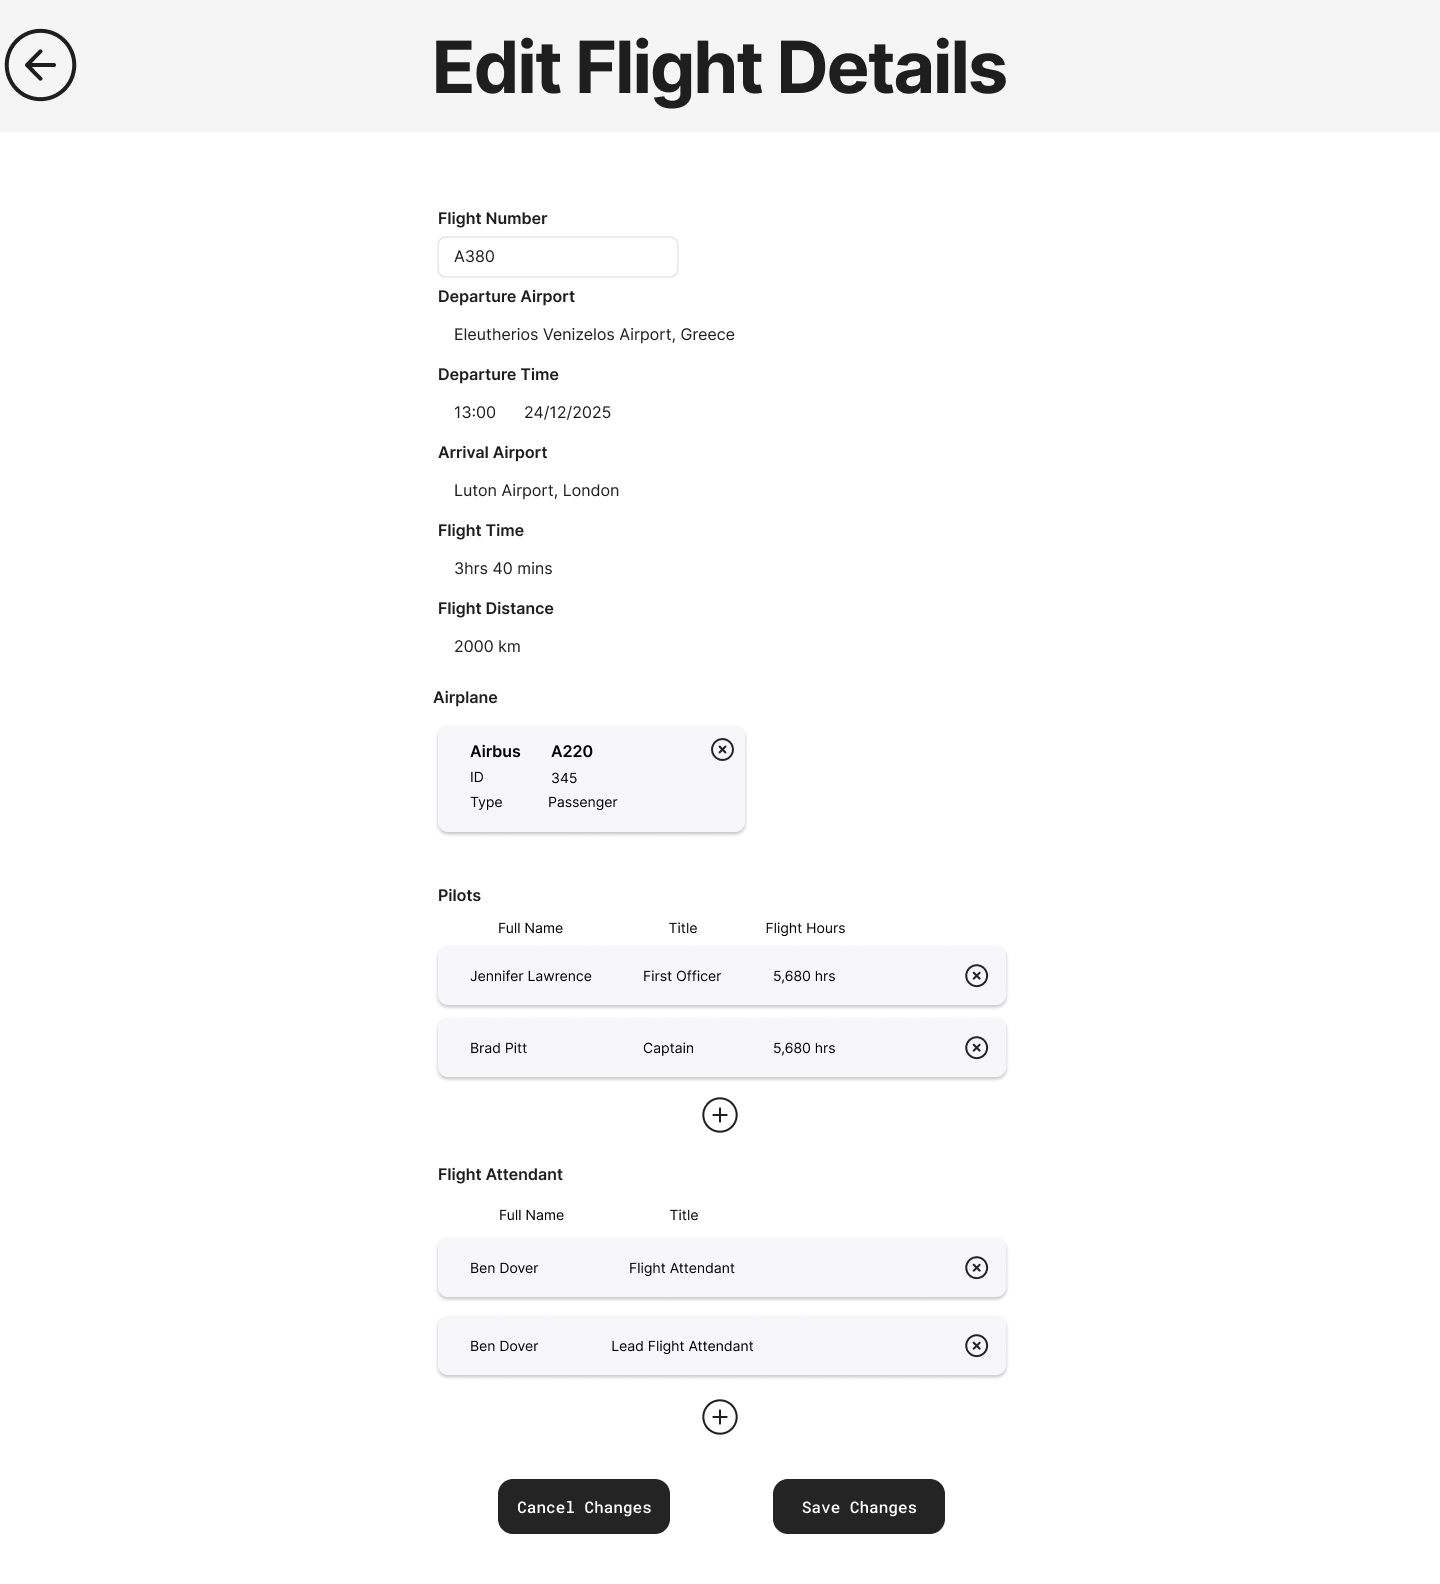
\includegraphics[width=0.5\textwidth]{../mockup-screens/flight-management/Flight-Edit.png}
		\caption{Edit Flight}
		\label{screen:Edit-Flight}
	\end{figure}


	\begin{figure}[H]
		\centering
		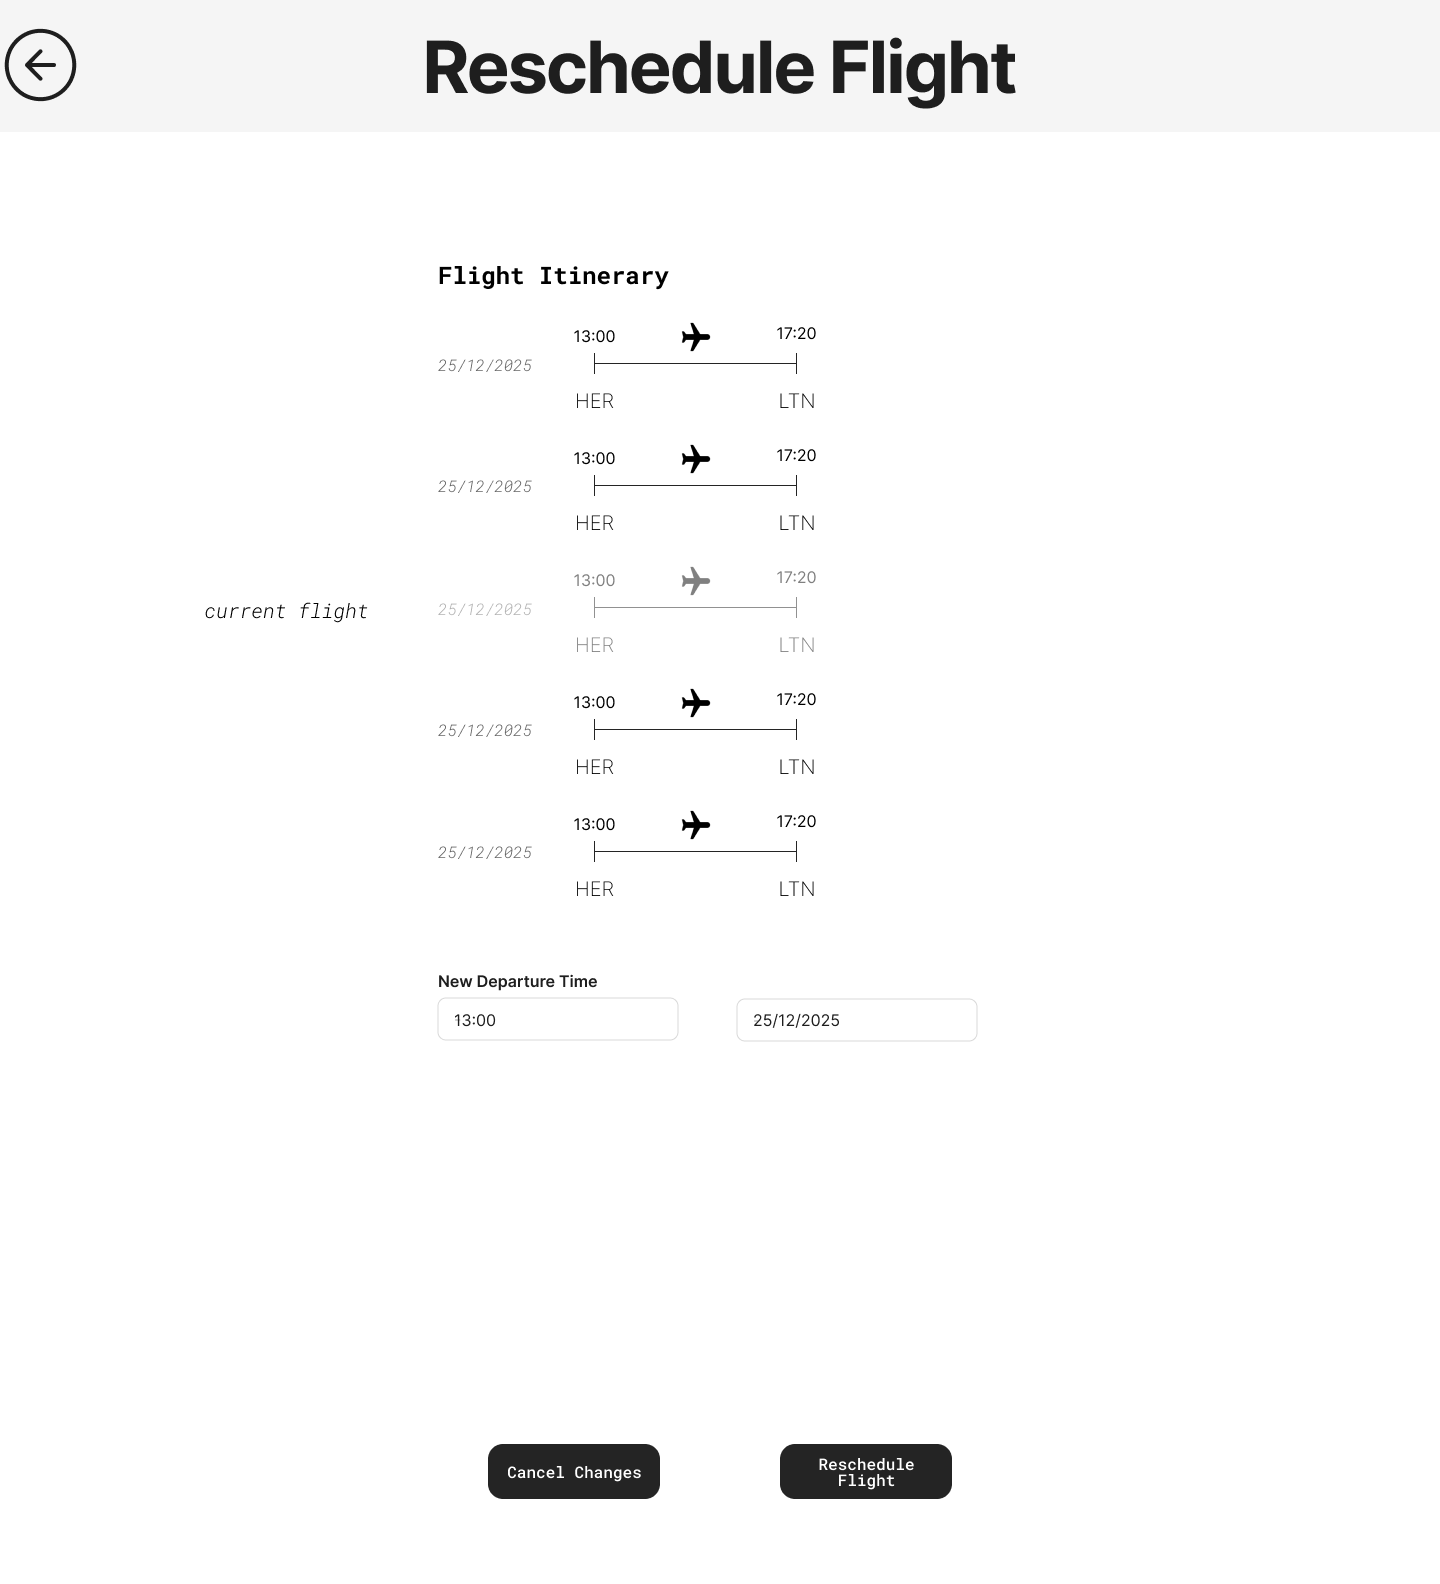
\includegraphics[width=0.5\textwidth]{../mockup-screens/flight-management/Flight-Reschedule.png}
		\caption{Flight Reschedule}
		\label{screen:Flight-Reschedule}
	\end{figure}
	
	\subsection{Διαχείριση Εργαζομένων}
	Το σύστημα προσφέρει τα ακόλουθα εργαλεία για τη διαχείριση των υπαλλήλων των αεροπορικών εταιρειών:
	\begin{enumerate}
		\item Τύποι εργαζομένων και αρμοδιότητες εργασίας: Πληροφορίες τηρούνται για τους πιλότους, τους αεροσυνοδούς, το προσωπικό εδάφους και τους ρόλους τους.
		\item Οι απαιτήσεις σε πλήρωμα καθορίζονται από το σύστημα, το οποίο λαμβάνει υπόψη τις αργίες και τις περιόδους ανάπαυσης κατά τον προσδιορισμό του αριθμού των μελών του πληρώματος που απαιτούνται για κάθε πτήση.
		\item Ανάθεση δρομολογίων: Οι εργαζόμενοι αντιστοιχίζονται με τα δρομολόγια ανάλογα με τα προσόντα τους, τη διαθεσιμότητα και τον χρόνο ανάπαυσης.
		\item Οι αναφορές για πιθανούς κινδύνους μπορούν να μεταφορτωθούν από τους πιλότους και προωθούνται αυτόματα στο αρμόδιο προσωπικό για αξιολόγηση.
	\end{enumerate}
	
	\subsection{Διαχείριση Αεροδρομίου}
	Το σύστημα διαχειρίζεται δεδομένα που σχετίζονται με το αεροδρόμιο, όπως:
	\begin{enumerate}
		\item Αποθήκευση δεδομένων αεροδρομίου: Η τοποθεσία, η χωρητικότητα και οι ανέσεις κάθε αεροδρομίου διατηρούνται σε αρχείο.
		\item Φιλτράρισμα πτήσεων με βάση τη διαδρομή: Μπορείτε να φιλτράρετε τις πτήσεις σύμφωνα με συγκεκριμένα δρομολόγια που συνδέουν διαφορετικά αεροδρόμια.
		\item Υπολογισμός συχνότητας πτήσεων: Με βάση τη ζήτηση, το σύστημα καθορίζει πόσες πτήσεις χρειάζεται κάθε αεροδρόμιο.
	\end{enumerate}
	
	\subsection{Κρατήσεις και Τιμές}
	Το σύστημα αναλύει τις τιμές των εισιτηρίων και βελτιστοποιεί τις στρατηγικές τιμολόγησης, όπως:
	\begin{enumerate}
		\item Ανάλυση τιμών εισιτηρίων: Χρησιμοποιώντας σύνολα δεδομένων (π.χ. τιμές πτήσεων από την Expedia), το σύστημα υπολογίζει τις μέσες τιμές εισιτηρίων και τις πωλήσεις για κάθε δρομολόγιο μηνιαίως.
		\item Υπολογισμός κόστους ανά μίλι: Το σύστημα υπολογίζει το μέσο κόστος ανά μίλι για κάθε πτήση.
		\item Εισαγωγή δεδομένων ανταγωνιστών: Οι διαχειριστές μπορούν να εισάγουν αρχεία CSV ή υπολογιστικά φύλλα που περιέχουν δεδομένα ανταγωνιστών ή αναμενόμενες τιμές εισιτηρίων για κάθε διαδρομή.
		\item Βελτιστοποίηση τιμολόγησης εισιτηρίων: Οι τιμές των εισιτηρίων προσαρμόζονται με βάση τα δεδομένα των ανταγωνιστών και τη ζήτηση.
	\end{enumerate}
	
	\subsection{Αναφορές}
	Το σύστημα δημιουργεί λεπτομερείς αναφορές για να βοηθήσει τους διαχειριστές να λάβουν τεκμηριωμένες αποφάσεις, όπως:
	\begin{enumerate}
		\item Στατιστικές αναφορές: Αναφορές σχετικά με διαδρομές, αναθέσεις αεροπλάνων, προγράμματα υπαλλήλων, χρόνους αναμονής και πολλά άλλα.
		\item Αναφορές PDF: Οι αναφορές δημιουργούνται αυτόματα σε μορφή PDF και αποστέλλονται μέσω ηλεκτρονικού ταχυδρομείου στο σχετικό προσωπικό.
		\item Αναφορές κινδύνου: Οι αναφορές που βασίζονται σε μεταφορτώσεις κινδύνων πιλότου δημιουργούνται και αποστέλλονται στο σχετικό προσωπικό.
	\end{enumerate}
	
	\subsection{Διαχείριση Φαγητού και Μενού}
	Το σύστημα διαχειρίζεται επιλογές φαγητού για διαφορετικούς τύπους πτήσεων, όπως:
	\begin{enumerate}
		\item Αποθήκευση επιλογών μενού φαγητού: Αποθηκεύονται λεπτομέρειες σχετικά με τις επιλογές φαγητού για διαφορετικούς τύπους αεροπλάνων και διάρκειες πτήσεων.
		\item Καθορισμός τιμών τροφίμων: Οι τιμές για κάθε τρόφιμο καθορίζονται με βάση τον τύπο του αεροπλάνου και τη διάρκεια της πτήσης.
	\end{enumerate}
	
	\subsection{Ανάθεση Βάρδιας Εργαζομένων}
	\begin{enumerate}
		\item Το σύστημα αντιστοιχίζει εργαζόμενους σε πτήσεις σύμφωνα με προσόντα, διαθεσιμότητα και κανονισμούς ανάπαυσης.
		\item Προγραμματίζει βάρδιες και ειδοποιεί τους υπαλλήλους.
	\end{enumerate}
	
	\subsection{Κατανάλωση Καυσίμων και Εκτίμηση Κόστος}
	\begin{enumerate}
		\item Υπολογίζει την κατανάλωση καυσίμων και το κόστος κάθε πτήσης.
		\item Παρέχει αναλύσεις για βέλτιστη διαχείριση κόστους.
	\end{enumerate}
	
	\subsection{Πρόβλεψη Τιμών Εισιτηρίων}
	\begin{enumerate}
		\item Ο χρήστης επιλέγει μια διαδρομή και ένα χρονικό διάστημα. 
		\item Το σύστημα ανακτά δεδομένα προηγούμενων πωλήσεων εισιτηρίων για την επιλεγμένη διαδρομή.
		\item Προσαρμόζει τις προβλέψεις με βάση εποχικότητα και τάσεις. 
		\item Παρουσιάζει προβλεπόμενες πωλήσεις εισιτηρίων ανά μήνα. 
		\item Ο χρήστης μπορεί να συγκρίνει τις προβλέψεις με προηγούμενες πωλήσεις. 
		\item Επιτρέπει στον διαχειριστή να ρυθμίσει την τιμολόγηση με βάση τη ζήτηση. 
		\item Οι προβλέψεις αποθηκεύονται για μελλοντική σύγκριση.  
	\end{enumerate}
	
	\subsection{Πρόσθετα Χαρακτηριστικά}
	Το σύστημα περιλαμβάνει επίσης χαρακτηριστικά όπως:
	\begin{enumerate}
		\item Παρακολούθηση συντήρησης αεροπλάνου: Παρακολούθηση χρονοδιαγραμμάτων συντήρησης και απαιτήσεων για κάθε αεροπλάνο.
		\item Παρακολούθηση της απόδοσης των εργαζομένων: Αποθήκευση και ανάλυση μετρήσεων απόδοσης των εργαζομένων.
		\item Διαχείριση χρόνων αναμονής: Παρακολούθηση και διαχείριση χρόνων αναμονής για αεροπλάνα και υπαλλήλους.
		\item Δημιουργία οικονομικών αναφορών: Δημιουργούνται αναφορές σχετικά με τα έσοδα, τα έξοδα και την κερδοφορία για να βοηθήσουν τους διαχειριστές να λαμβάνουν αποφάσεις βάσει δεδομένων.
	\end{enumerate}
	
	\section{Οφέλη του Συστήματος}
	\begin{enumerate}
		\item Αποδοτικότητα: Οι βελτιστοποιημένες διαδρομές και η κατανομή πόρων μειώνουν το λειτουργικό κόστος και βελτιώνουν την αποδοτικότητα.
		\item Ακρίβεια: Οι αυτοματοποιημένοι υπολογισμοί και αναφορές διασφαλίζουν την ακριβή ανάλυση δεδομένων.
		\item Ευελιξία: Το σύστημα μπορεί να προσαρμοστεί σε διαφορετικά μεγέθη αεροπορικών εταιρειών και επιχειρησιακές ανάγκες.
		\item Φιλικό προς το χρήστη: Ένα ασφαλές σύστημα σύνδεσης και έλεγχος πρόσβασης βάσει ρόλων καθιστούν το σύστημα εύκολο στη χρήση για όλους τους υπαλλήλους.
	\end{enumerate}
	
	\subsection{Περιφερειακά και Συσκευές}
	Το SkyOps είναι σχεδιασμένο να λειτουργεί σε ποικίλες συσκευές, όπως:
	\begin{enumerate}
		\item Υπολογιστές γραφείου και φορητούς υπολογιστές. 
		\item Tablets και κινητές συσκευές για πρόσβαση εν κινήσει.
		\item Εκτυπωτές για εκτύπωση αναφορών και εισιτηρίων.  
		\item Εξοπλισμό ασφαλείας, όπως συστήματα ελέγχου πρόσβασης για επαλήθευση ταυτότητας εργαζομένων.   
	\end{enumerate}
	
	\section{Shareholders}
	Το σύστημα υποστηρίζει τη διαχείριση μετόχων παρέχοντας οικονομικές αναφορές και
	στατιστικά στοιχεία που αφορούν την απόδοση της αεροπορικής εταιρείας.
	Οι μέτοχοι μπορούν να έχουν πρόσβαση σε αναφορές εσόδων,
	κόστους λειτουργίας και προβλέψεων για την κερδοφορία.
	
	
	\section{Συμπέρασμα}
	Το SkyOps είναι ένα ισχυρό εργαλείο για τις 
	αεροπορικές εταιρείες που επιθυμούν να βελτιστοποιήσουν τις 
	δραστηριότητές τους, να μειώσουν το κόστος και να βελτιώσουν 
	την ποιότητα των υπηρεσιών. Αυτοματοποιώντας πολύπλοκες 
	διαδικασίες και παρέχοντας λεπτομερείς πληροφορίες, το σύστημα 
	βοηθά τις αεροπορικές εταιρείες να παραμείνουν ανταγωνιστικές 
	σε έναν κλάδο με γρήγορους ρυθμούς.
	
\end{document}